\documentclass[12pt,twoside]{article}

% *** Set page dimensions ***
\raggedbottom
\parindent=0in
%\setlength{\topmargin}{-0.5in}
%\setlength{\oddsidemargin}{0.1875in}
%\setlength{\evensidemargin}{0in}
%\setlength{\textheight}{8.5in}
%\setlength{\textwidth}{6.225in}
%\addtolength{\oddsidemargin}{-0.7in}
%\addtolength{\evensidemargin}{-1.2in}
%\setlength{\oddsidemargin}{-0.2in}
%\setlength{\evensidemargin}{-0.2in}
%\addtolength{\textwidth}{1.4in}
%\addtolength{\topmargin}{-.875in}
%\addtolength{\textheight}{2.00in}

% *** Packages ***
\usepackage{alltt}
\usepackage{tocloft}
\usepackage{graphicx}
\usepackage{lscape}
\usepackage{amssymb}
\usepackage{float}
\usepackage{amsmath}
\usepackage{gensymb}
%\usepackage{subfigure}
\usepackage{lscape}
\usepackage{epsfig}
\usepackage{enumerate}
\usepackage{multicol}
\usepackage{fancyhdr}
\usepackage{epstopdf}
\usepackage{hyperref}
\usepackage{listings}

% *** Table of contents and Sectioning *** 
\setcounter{secnumdepth}{0}
\setcounter{tocdepth}{5}

% *** Table of contents and Sectioning *** 
\newcommand{\next}{\addtocounter{enumi}{9} \item}
\newcommand{\now}[1]{\setcounter{enumi}{#1}}
\newcommand{\Z}{\mbox{\sf Z\hspace{-1.5mm}Z}}
\newcommand{\R}{\mbox{\rm I\hspace{-0.75mm}R}}
\columnsep=0.75in

% *** Shortcuts for syntax ***
\newcommand{\ds}{\displaystyle }
\newcommand{\vsc}{\vspace{4mm}}
\newcommand{\dd}[1]{\frac{d}{d{#1}} \,} 
\newcommand{\ddx}{\frac{d}{dx} \,} 
\newcommand{\ddy}{\frac{d}{dy} \,} 
\newcommand{\ddz}{\frac{d}{dz} \,} 
\newcommand{\dydx}{\frac{dy}{dx} \,} 
\newcommand{\dydt}{\frac{dy}{dt} \,} 
\newcommand{\dfdx}{\frac{df}{dx} \,} 
\newcommand{\ddt}[1]{  \frac{d{#1}}{dt} }
\newcommand{\pp}[2]{  \frac{\partial{#1}}{\partial {#2}} }
\newcommand{\zx}{\frac{\partial z}{\partial x} \,}
\newcommand{\zy}{\frac{\partial z}{\partial y} \,}
\newcommand{\limh}{\lim_{h \rightarrow 0} \;}
\newcommand{\diff}{\frac{d}{dx} \,}
\newcommand{\de}{\Delta}
\renewcommand{\thesection}{\Roman{section}}
\newcommand{\bfr}{\begin{flushright}}
\newcommand{\efr}{\end{flushright}}
\newcommand{\dx}{\frac{\partial f}{\partial x} \,}
\newcommand{\dy}{\frac{\partial f}{\partial y} \,}
\newcommand{\p}{\partial}
\newcommand{\vi}{\vec{i}}
\newcommand{\vj}{\vec{j}}
\newcommand{\vk}{\vec{k}}
\newcommand{\lan}{\left\langle}
\newcommand{\ran}{\right\rangle}
\newcommand{\reading}[1] { {\em Reading: #1}}
\renewcommand{\Pr}{ \mbox{Pr}}

% *** Commands related to textbook references
\newcommand{\problem}{{\bf Problem.} }

% *** Footnoting with symbols ***
\long\def\symbolfootnote[#1]#2{\begingroup%
\def\thefootnote{\fnsymbol{footnote}}\footnote[#1]{#2}\endgroup}

% *** Defining a boxed note ***
\floatstyle{boxed}
\newfloat{noteinbox}{htb}{loa}
\newenvironment{boxnote}{\begin{noteinbox}[H]}{\end{noteinbox}}

\newcommand{\Question}{ {\bf Question: }  }
\newcommand{\Example}[1]{ {\bf Example: } {\em #1} }
\newcommand{\ExampleCont}[1]{ {\em #1} }

% *** Define the boxed Week #/summary at the beginning/end of every chapter ***
\newcommand{\sectionbox}[1]{% 
\begin{tabular}{|p{6in}|}%
\hline%
\ \\ %
{\Large {\bf {#1}}}  \\%
\ \\%
\hline%
\end{tabular}}

% *** Shortcuts *** 
\newcommand\goals{\large {\bf {Goals:}}}
\newcommand\setfont{ }

% *** Week commands: overwritten in each notes file
\newcommand{\Week}{Null-InPreambleCommon}
\newcommand{\WeekTitle}{Null-InPreambleCommon}
\newcommand{\Course}{MNTC P04}
\newcommand{\SetNum}{1 }
\newcommand{\topic}[1]{
\newpage
\setcounter{page}{1}
\fancyhead[LE,RO]{#1 - \thepage}
}

% *** Setup Latex for the large version of the files ***
%\usepackage[landscape]{geometry}
\usepackage[letterpaper,landscape,hmargin={.8in,.8in},vmargin={1in,0.2in}]{geometry}

% Remove paragraph indents
\setlength{\parindent}{0pt}

% Spacing at the top for the header is too large by default
\setlength{\voffset}{-5ex}

% **** RENEW SCALING COMMANDS HERE ****
% *** Text in boxes ***
\renewenvironment{boxnote}{\begin{noteinbox}[H] \huge}{\end{noteinbox}} 

% *** Chapter lead in/summary boxes ***
\renewcommand{\sectionbox}[1]{% 
\begin{tabular}{|p{9.5in}|}%
\hline%
\ \\ %
{\huge {\bf {#1}}}  \\%
\ \\%
\hline%
\end{tabular}}

% *** 'Section'' commands, which are sometimes used for spacing
% From http://zoonek.free.fr/LaTeX/LaTeX_samples_section/0.html
\makeatletter
 \renewcommand\section{\@startsection {section}{1}{\z@}%
                                    {-3.5ex \@plus -1ex \@minus -.2ex}%
                                    {0.3ex \@plus.2ex}%
                                    {\setfont\bf}}

 \renewcommand\subsection{\@startsection {subsection}{1}{\z@}%
                                    {-3.5ex \@plus -1ex \@minus -.2ex}%
                                    {0.3ex \@plus.2ex}%
                                    {\setfont\bf}}

% *** 'Goals' should be larger in the overheads ***
\renewcommand\goals{\huge {\bf {Goals:}}}
\renewcommand\setfont{\huge }

\thispagestyle{empty}

\setfont 

\newcommand{\WeekTitleOne}{Derivatives - Foundations}
\newcommand{\WeekTitleTwo}{Derivatives - Linearization and Applications}
\newcommand{\WeekTitleThree}{Derivatives - Modeling}
\newcommand{\WeekTitleFour}{Integrals - Foundations}
\newcommand{\WeekTitleFive}{Integrals - Techniques}
\newcommand{\WeekTitleSix}{Integrals - Modeling}
\newcommand{\WeekTitleSeven}{Differential Equations - }
\newcommand{\WeekTitleEight}{Differential Equations - }
\newcommand{\WeekTitleNine}{Differential Equations - }
\newcommand{\WeekTitleTen}{Linear Algebra - }
\newcommand{\WeekTitleEleven}{Linear Algebra - }
\newcommand{\WeekTitleTwelve}{Linear Algebra - }



\begin{document}
\setfont
\pagestyle{fancy}
\renewcommand{\Week}{1 }
\renewcommand{\WeekTitle}{\WeekTitleOne }

\fancyhead[LE,RO]{Week \Week}  % default, usually only for first page
\fancyfoot{}
\sectionbox{Week \#\Week: \WeekTitle}


\vspace{5mm}
\goals
\begin{itemize}
\item Interpret the derivative, and be able to discuss the difference
  between the secant line and the derivative 
\item Compute the derivative of polynomial, exponential, logarithmic,
  powers, trigonometric functions and their combinations, with the
  correct application of the product and quotient rules, and the chain
  rule 
\item Report the graphs, domain and range of the inverse trigonometric
  functions arcsin, arccos and arctan.
\item Apply the derivative rules for arcsin, arccos and arctan.
 \end{itemize}

\vspace{5mm}

% topics
% 2.6 - give examples of functions which are and are NOT differentiable.
%  - graphical and formula
 
 
\newpage

\topic{Introduction}
\subsection*{Introduction}

The two fundamental ideas in calculus are:
\begin{itemize}
\item The {\bf derivative}, which gives the rate of change of a function, and \\[2ex]
\item The {\bf integral}, which computes the total accumulation based
  on a rate.
\end{itemize}

\newpage

Many fundamental quantities in physics are
related through derivatives and integrals.  For example: \\

\begin{center}
  {\bf Position} \\[10ex]
  {\bf Velocity} \\[10ex]
  {\bf Acceleration} 
\end{center}

\newpage


\newpage

We will spend the first half of this course examining differential
calculus and integral calculus.  \\[2ex]

The assumption for the derivative section is that the fundamental
ideas will be review, so the pace will be fairly aggressive.  We will
also start including some calculations and graphical analysis using MATLAB.  \\[2ex]

Take advantage of the practice problems to practice your skills, and
get in touch with the instructor if you need any help.



\newpage
\topic{Differential Calculus - Slopes, Secants and the Derivative}
\subsection*{Slopes, Secants and the Derivative}
A {\bf secant line} is a line connecting any two points on a graph.
\vfill

The {\bf slope of a secant line} gives 
\begin{itemize}
\item the {\bf average rate of change} of $f(x)$ over some interval $\Delta x$.
\item the {\bf average velocity} over an interval, if $f(t)$ represents {\bf position}.
\item the {\bf average acceleration} over an interval, if $f(t)$ represents {\bf velocity}.
\end{itemize}
\problem Give the units of the slope of a secant line.

\vspace{1in}

\newpage

The {\bf derivative} gives the {\bf slope of a tangent line} at a {\bf
  single point} on a graph.

\vfill

The derivative gives:
\begin{itemize}
\item the {\bf limit of the average slope} as the interval $\Delta x $ approaches zero.
\item the {\bf instantaneous rate of change} of $f(x)$.
\item the {\bf velocity}, if $f(t)$ represents {\bf position}.
\item the {\bf acceleration}, if $f(t)$ represents {\bf velocity}.
\end{itemize}

\problem Give the units of the derivative.
\vspace{1in}

\newpage

\topic{Differentiability}

\section*{Differentiability}


The definition of the derivative is based on the classic
$\ds \left(\frac{\mbox{rise}}{\mbox{run}}\right)$ formula for slopes.

\begin{align*} 
  f'(x) = \frac{d}{dx} f = \dfdx = \lim_{\Delta x \to 0} \frac{\Delta f}{\Delta x} = \lim_{h \to 0} \frac{f(x+h) - f(x)}{h}
\end{align*} 

\newpage

A function $f$ is {\bf{differentiable}} at a given point $a$ if it has
a derivative at $a$, or the limit above exists.  There is also a
graphical interpretation differentiability: {\bf{if the graph has a
    unique and finite slope at a point}}.  Since the slope in question
is automatically the slope of the tangent line, we could also say that

\begin{quote} {\sc{$f$ is differentiable at $a$ if its graph has a
      (non-vertical) tangent at $(a,f(a))$}}.
\end{quote}

\vfill

For functions of the form $y = f(x)$, we do not consider points with
vertical tangent lines to have a real-valued derivative, because a
vertical line does not have a finite slope.

\vsc
\newpage


Here are the ways in which a function can fail to be differentiable at a point $a$:
\begin{enumerate}
\item The function is not continuous at $a$.
\item The function has a corner (or a cusp) at $a$.
\item The function has a vertical tangent at $(a,f(a))$.
\end{enumerate}

\problem Sketch an example graph of each possible case.

\vfill

\newpage

{\bf Reminder: Differentiability is Common}

You will notice that, despite our concern about some functions {\em
  not} being differentiable, most of our standard functions
(polynomials, rationals, exponentials, logarithms, roots) {\bf are}
differentiable at most points.  Therefore we should investigate what
all these possible derivative/slope values could tell us.

\vspace{0.5in}

\topic{Interpreting the Derivative}

{\bf Interpreting the Derivative}


\begin{boxnote}

\begin{itemize}
\item Where $f'(x) > 0$, or the {\bf derivative is positive}, \\
  $f(x)$ is {\bf increasing}. \\[1ex]
\item Where $f'(x) < 0$, or the {\bf derivative is negative}, \\
  $f(x)$ is {\bf decreasing}. \\[1ex]
\item Where $f'(x) = 0$, or the {\bf tangent line to the graph is
    horizontal}, $f(x)$ has a {\bf critical point}.
\end{itemize}
\end{boxnote}

\newpage

\problem Consider the graph of $f(x)$ shown below. 

\begin{tabular}{ll}
\begin{minipage}{5in}
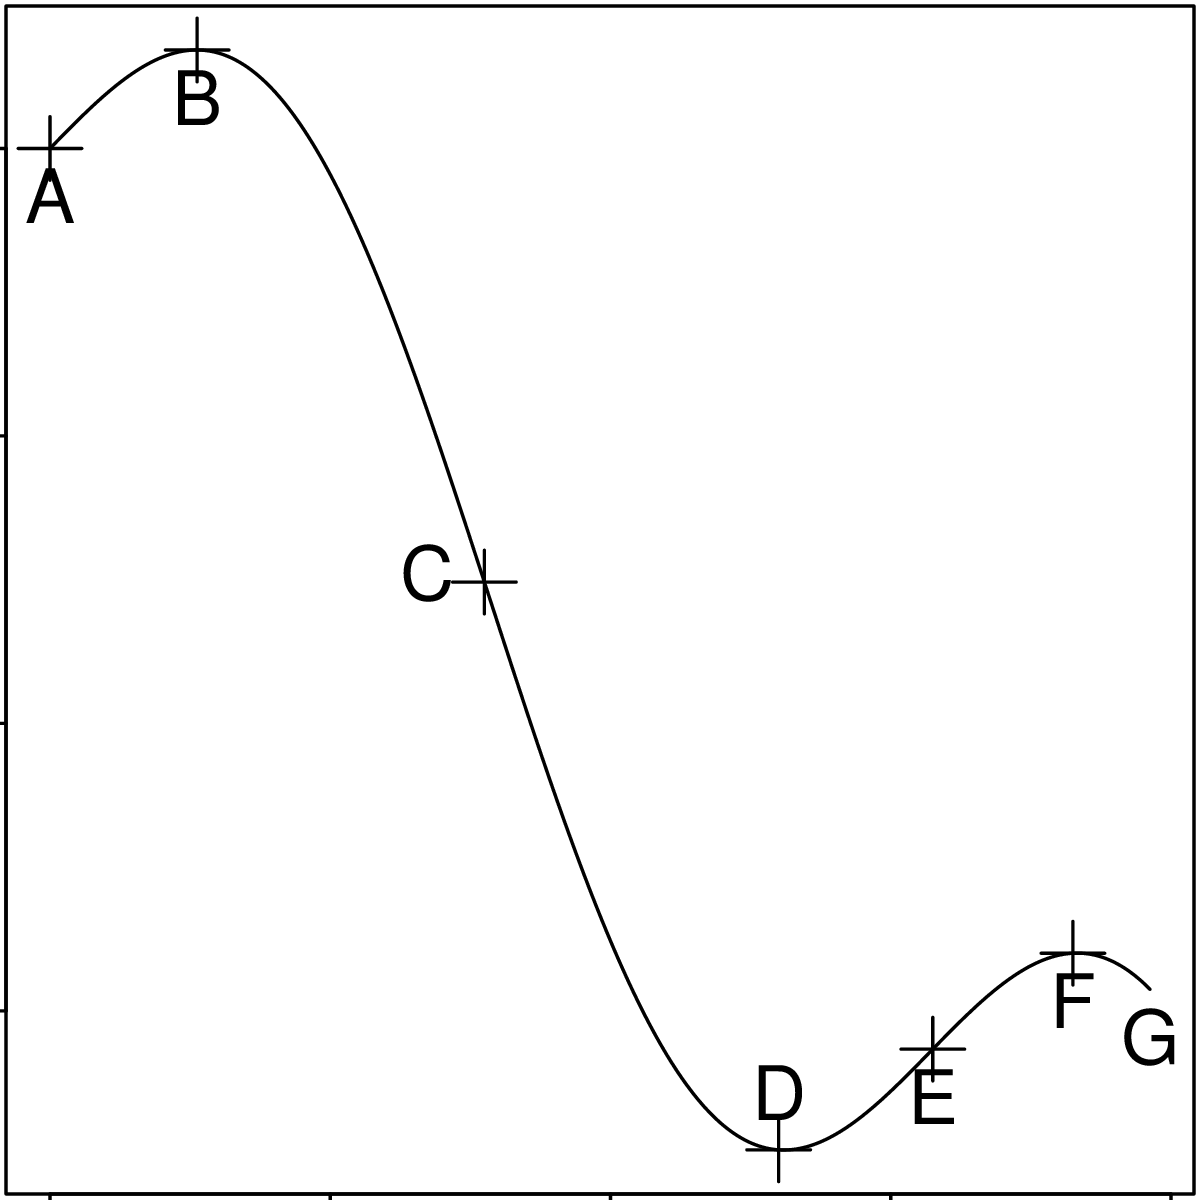
\includegraphics[width=5in]{graphics/notes_01_incr_decr}
\end{minipage} &
\begin{minipage}{4.5in}
On what intervals is $f'(x) > 0$?
\end{minipage}
\end{tabular}

\newpage

\begin{tabular}{ll}
\begin{minipage}{5in}
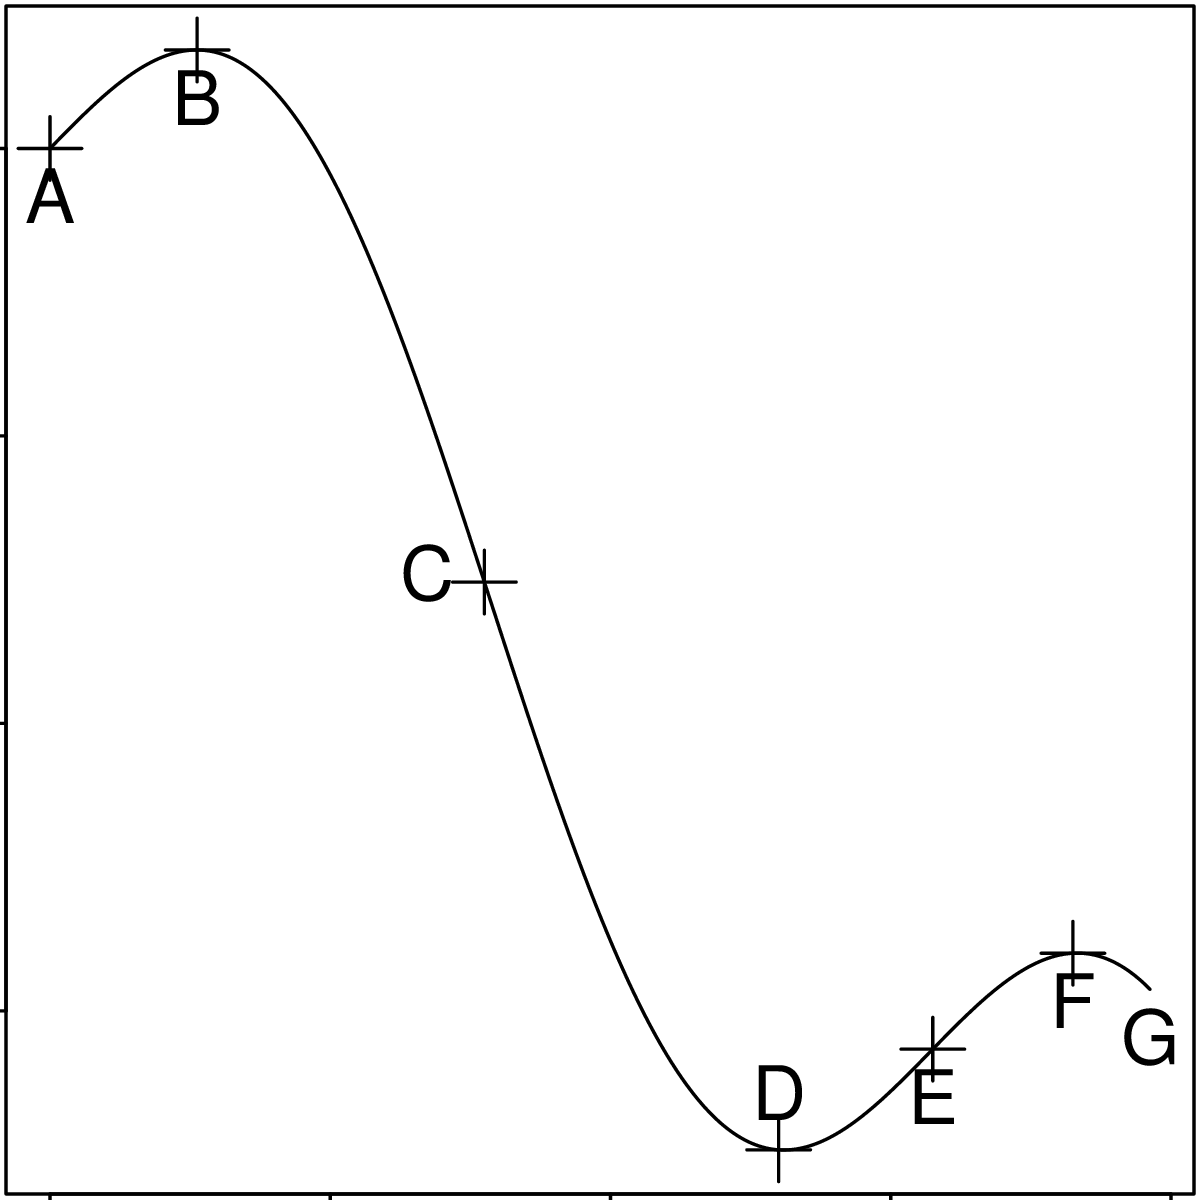
\includegraphics[width=5in]{graphics/notes_01_incr_decr}
\end{minipage} &
\begin{minipage}{4.5in}
\problem Where does $f'(x)$ takes on its {\bf largest negative value}?
\end{minipage}
\end{tabular}


\newpage

\topic{Graphs of the Derivative}

\section*{Graphs, and Graphs of their Derivatives}


\problem Consider the same graph again, and the graph of its derivative.
Identify important features that associate the two. 

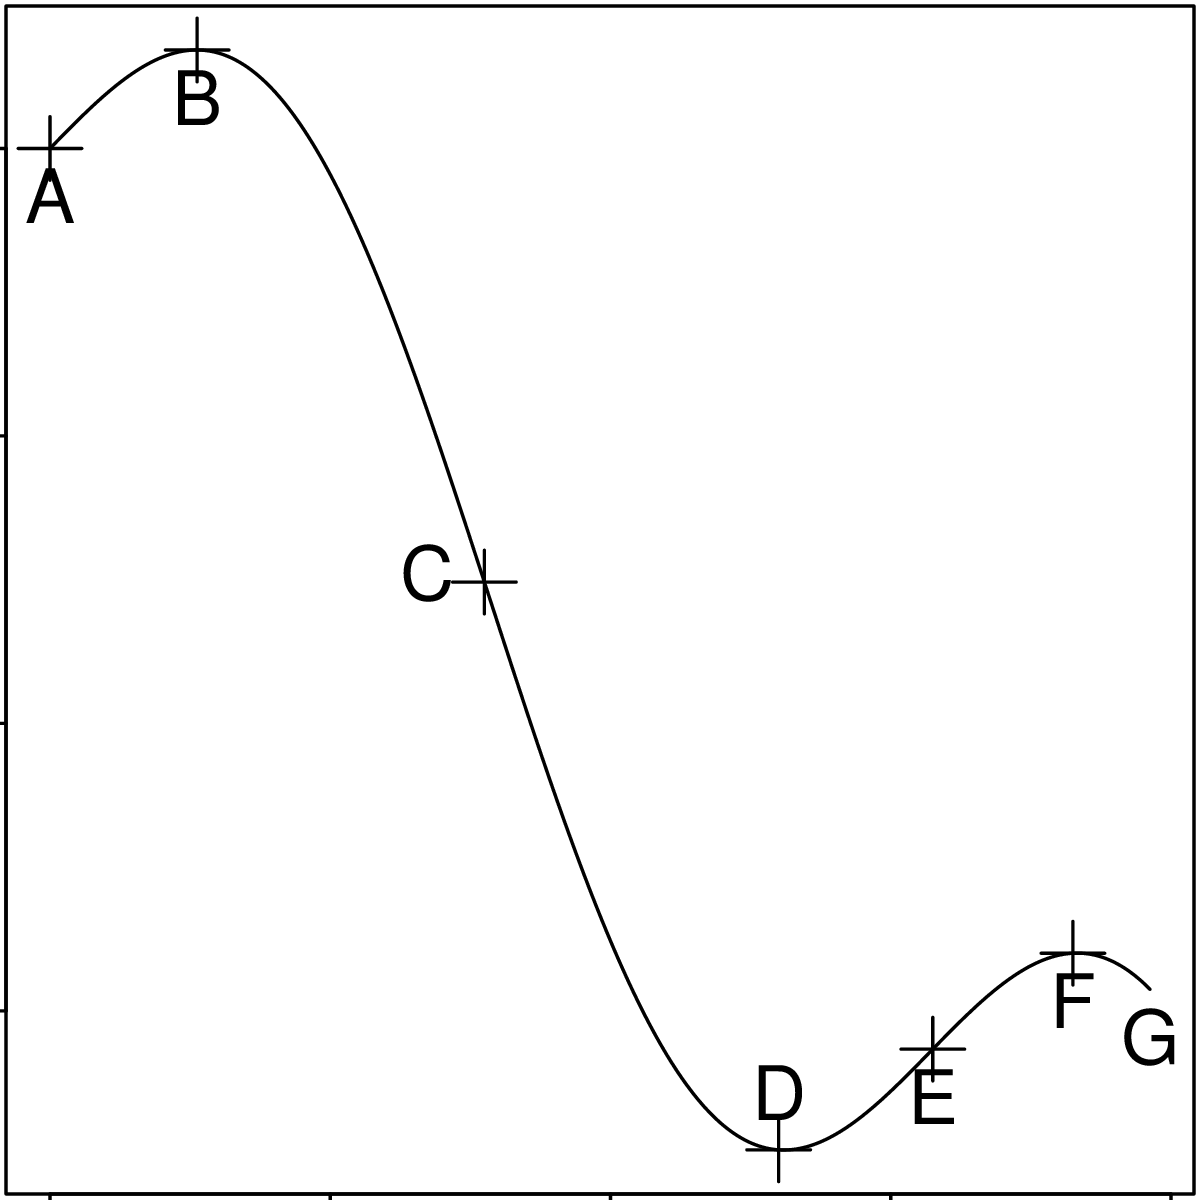
\includegraphics[width=2.9in]{graphics/notes_01_incr_decr} \\[.1in]
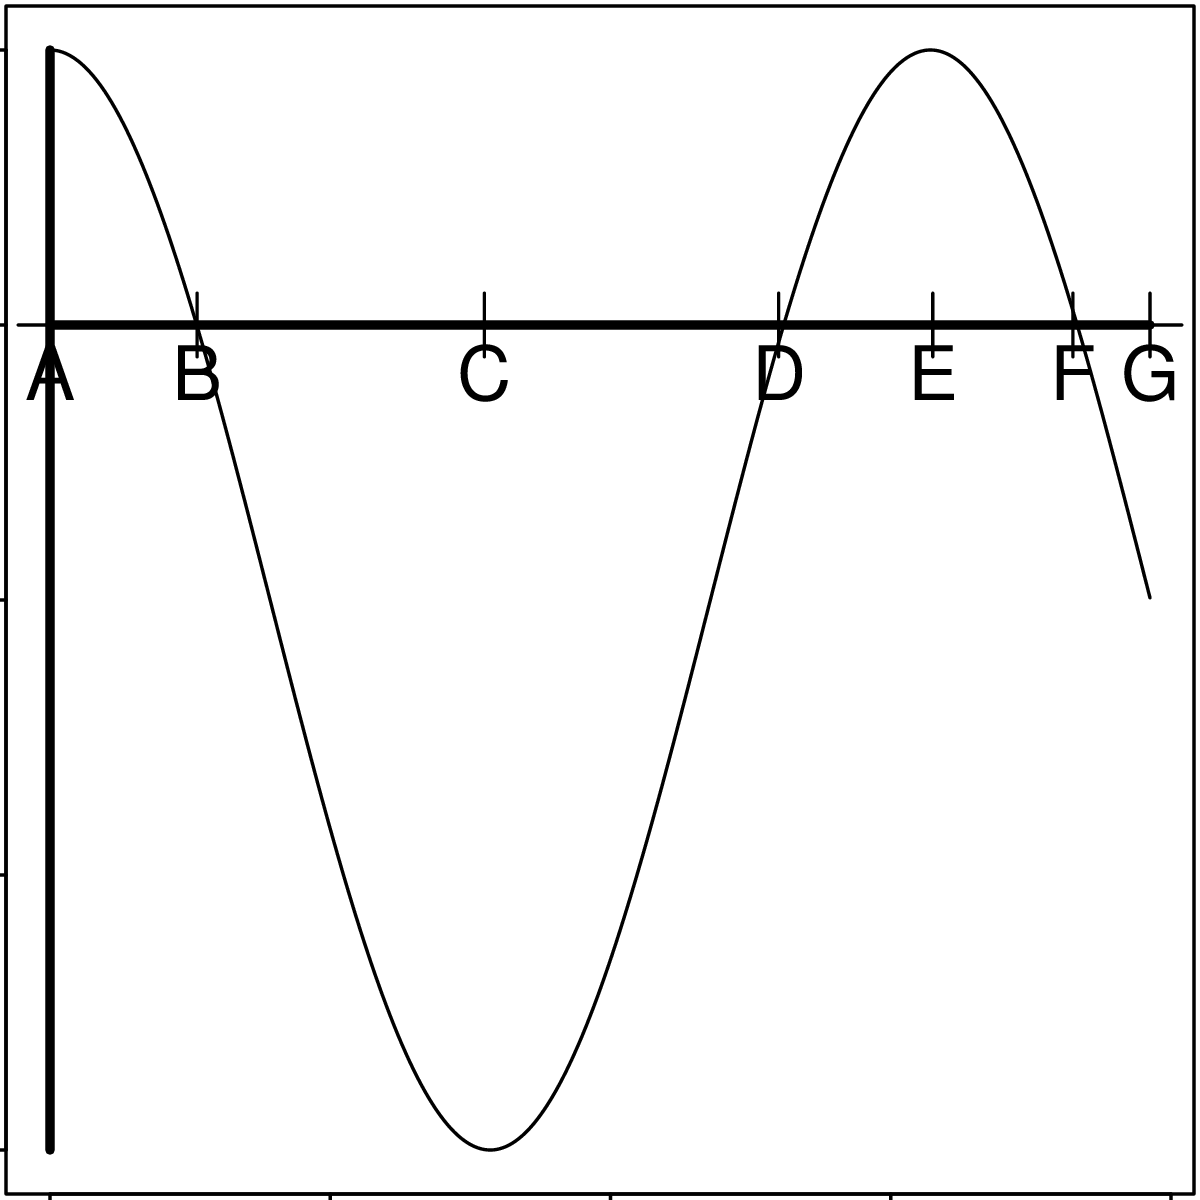
\includegraphics[width=2.9in]{graphics/notes_01_incr_decr_deriv}

\newpage

\problem  Consider the graph of $f(x)$ shown:

\begin{minipage}[h]{0.3\linewidth}
\begin{center}
  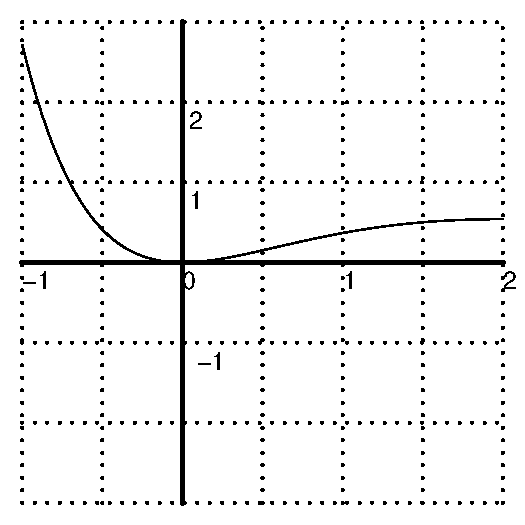
\includegraphics[width=1.0\linewidth]{graphics/notes_01_f_and_deriv_graph_f} \\
  $f(x)$
\end{center}
\end{minipage}
\begin{minipage}[h]{0.65\linewidth}
\begin{center}
\begin{tabular}{cc}
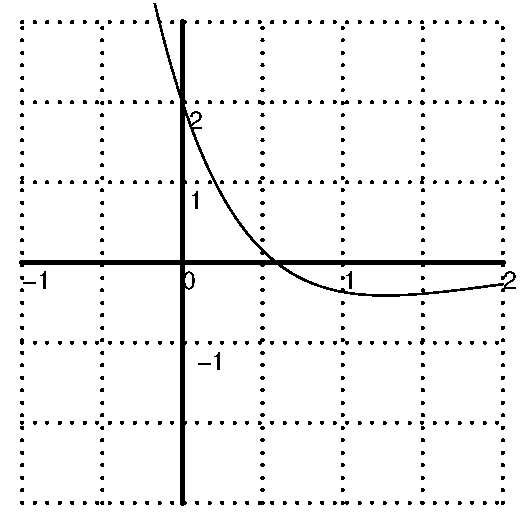
\includegraphics[width=2.5in]{graphics/notes_01_f_and_deriv_graph_c} &
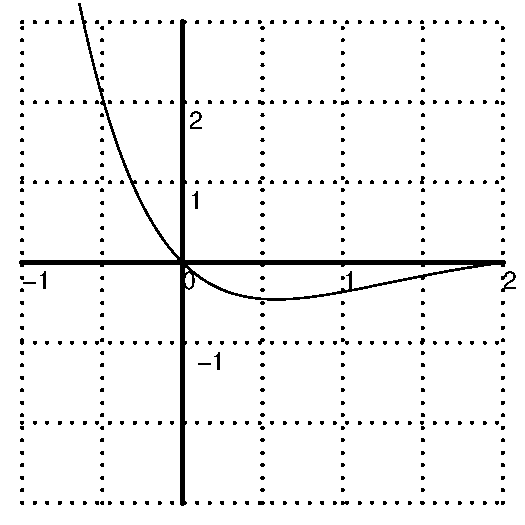
\includegraphics[width=2.5in]{graphics/notes_01_f_and_deriv_graph_b} \\
{\bf A} &  {\bf B} \\ \hline
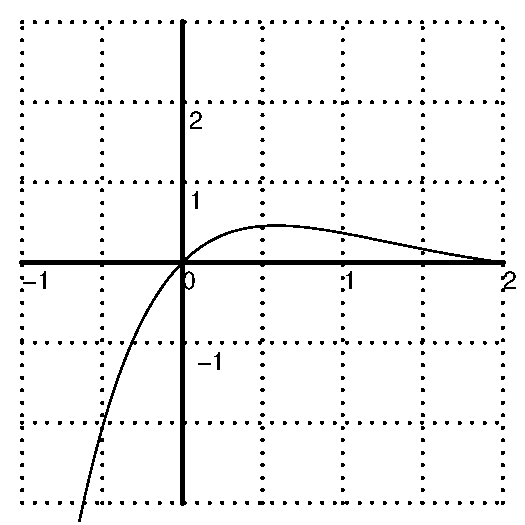
\includegraphics[width=2.5in]{graphics/notes_01_f_and_deriv_graph_a} &
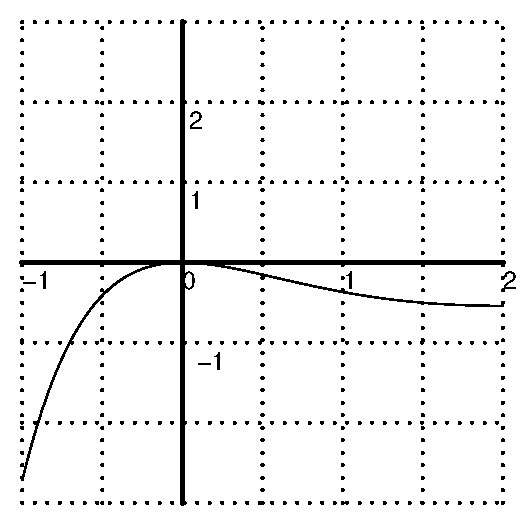
\includegraphics[width=2.5in]{graphics/notes_01_f_and_deriv_graph_d} \\
{\bf C} &  {\bf D} 
\end{tabular}
\end{center}
\end{minipage}

Which of the graphs on the right is the graph of the {\bf derivative} of
$f(x)$?
\newpage

\topic{Computing Derivatives - Basic Formulas}

\section*{Computing Derivatives}
% {\bf Note:} The standard formulas for derivatives are covered in the
% Grade 12 Ontario curriculum. While they will be reviewed here, {\bf
%   students who are not familiar with them should begin both textbook
%   reading and the assignment problems for this unit as soon as
%   possible.}



Beyond the graphical interpretation of derivatives, there are all the
algebraic rules.  {\bf All of these rules} are based on the {\bf definition}
of the derivative, \\[2ex]
\begin{align*} 
f'(x) = \frac{d}{dx} f = \dfdx = \lim_{\Delta x \to 0} \frac{\Delta f}{\Delta x} = \lim_{h \to 0} \frac{f(x+h) - f(x)}{h}
\end{align*}  \\[2ex]

However, by finding common patterns in the derivatives of certain
families of functions, we can compute derivatives much more quickly
than by using the definition.

\newpage

\begin{boxnote}
{\bf Sums, Powers, and Differences}

\LARGE
\begin{tabular}{lc}
Constant Functions: & $\ds \ddx k = 0 $ \\[7ex]
Power rule: & $\ds \ddx x^p = p x^{p-1}$ \\[7ex]
Sums : & $\ds \ddx f(x) + g(x) = \left(\ddx f(x)\right) + \left(\ddx g(x) \right)$ \\[7ex]
Differences: & $\ds \ddx f(x) - g(x) = \left(\ddx f(x)\right) - \left(\ddx g(x) \right)$ \\[7ex]
Constant Multiplier: & $\ds \ddx \left[k f(x)\right] = k \left(\ddx f(x)\right)$, so long as $k$ is a constant
\end{tabular}
\setfont

\end{boxnote}

\newpage

\problem Evaluate the following derivatives: 

$\ds \ddx \left(x^{5} - 2 x\right)$

\vfill

$\ds \ddx \left(4.1 \sqrt{x} + \frac{4}{x}\right)$

\vfill

\newpage
{\bf Question: } The derivative of $\ds -3t^2 - \frac{1}{t^2}$ is 

\begin{enumerate}
\item $\ds -6 t^3 + 2 \frac{1}{t^3} $ \\[1ex]
\item $\ds -6 t + 2 \frac{1}{t^3} $ \\[1ex]
\item $\ds -6 t - 2 \frac{1}{t^3} $ \\[1ex]
\item $\ds -t^3 + 2 \frac{1}{t} $
\end{enumerate}

\newpage

\begin{boxnote}
{\bf Exponentials and Logs}
\begin{center}
\begin{tabular}{lp{0.2in}l}
$e$ as a base: && $\ds \ddx e^x = e^x $ \\[7ex]
Other bases: && $\ds \ddx a^x = a^x (\ln(a))$ \\[7ex]
Natural Log: && $\ds \ddx \ln(x) = \frac{1}{x}$ \\[7ex]
Other Logs: &&$\ds \ddx \log_a(x) = \frac{1}{x} \frac{1}{\ln(a)}$ \\[7ex]
\end{tabular}
\end{center}
\end{boxnote}

\newpage

\problem Evaluate the following derivatives:

$\ds \ddx \left( 3 \cdot 10^x + 10 \cdot x^3  \right)$

\vfill

$\ds \ddx \left( e^x + \log_{10}(x) \right)$

\vfill

(Exponential and log derivatives are relatively straightforward, until
we mix in the product, quotient, and chain rules.)

\newpage

\topic{Computing Derivatives - Product and Quotient Rules }

\begin{boxnote}
{\bf Product and Quotient Rules}

\begin{center}
\begin{tabular}{lc}
  Products: & \LARGE $\ds \ddx f(x) \cdot g(x) = f'(x) g(x) + f(x) g'(x)$ \\[1in]
  Quotients: &\LARGE  $\ds \ddx \frac{f(x)}{g(x)} = \frac{f'(x) g(x) - f(x) g'(x)}{\left(g(x) \right)^2}$ \\ 
\end{tabular}
\end{center}



\end{boxnote}

\problem Evaluate the following derivatives: 

$\ds \ddx \left( 2.1 x^4 \ln(x) \right)$

\vfill

\newpage

$\ds \ddx \left( \frac{\sqrt{x}}{e^x} \right)$

\vfill

$\ds \ddt{} \left( 7 t^3 2^t \right)$

\vfill

\newpage
{\bf Question: } The derivative of $\ds \frac{10^x}{x^3}$ is 

\begin{enumerate}[(a)]
\item $\ds   \frac{10^x}{\ln(10)} x^{-3} + 10^x (-3 x^{-4})$  \\[3ex]
\item $\ds \frac{10^x \ln(10) x^3  - 10^x (3x^2)} {x^6}$ \\[3ex]
\item $\ds  \frac{10^x \frac{1}{\ln(10)} x^3  - 10^x (3x^2)} {x^6}$ \\[3ex]
\item $\ds  \ln(10) 10^x x^{-3} + 10^x (-3 x^{-4})$  \\[3ex]
\end{enumerate}

\newpage

\topic{Computing Derivatives - Chain Rule}

\begin{boxnote}
{\bf Chain Rule}

\begin{center}
\begin{tabular}{lc}
Nested Functions: & \LARGE $\ds \ddx \left[ f(g(x)) \right] = f'(g(x))\cdot g'(x)$  \\
~\\[1in]

Liebnitz form & \LARGE $\ds \ddx f(g(x)) = \frac{df}{dg} \frac{dg}{dx}$ \\
\end{tabular}
\end{center}
\end{boxnote}

\newpage 

\problem Evaluate the following derivatives: 

$\ds \ddt{} e^{t^4}$ 

\vfill

\newpage

$\ds \ddx  \ln( 1+ \sqrt{x}) $

\vfill

\newpage
$\ds \ddx \left( \frac{1}{\ln(x)+x^3} \right)$

\vfill

\newpage

$\ds \ddt{} \left( e^{5t-1} + 10^{3t} \right)$

\vfill

\newpage
{\bf Question: } The derivative of $\ds e^{\sqrt{x}}$ is 

\begin{enumerate}[(a)]
\item $\ds  \frac{1}{2} e^{\frac{1}{\sqrt{x}}}$ \\[1ex]
\item $\ds e^{\sqrt{x}} \left(\sqrt{x}\right)$  \\[1ex]
\item $\ds \frac{1}{2} e^{\sqrt{x}} \left(\frac{1}{\sqrt{x}}\right)$ \\[1ex]
\item $\ds \frac{1}{2} e^{\sqrt{x}} \left(\sqrt{x}\right)$
\end{enumerate}

\vfill

\newpage

\topic{Computing Derivatives - Trigonometric Functions}


\subsection*{Derivatives of Trigonometric Functions}
\begin{boxnote}
$$ \ds \diff \sin( x) = \cos (x)$$ \\[-2.0ex]
$$ \ds \diff \cos( x) = - \sin (x)$$ \\[-2.0ex]
$$ \ds \diff \tan(x) = \sec^2 (x)$$ \\[-2.0ex]
$$ \ds \diff \sec(x) = \sec(x)\tan(x)$$ \\[-2.0ex]
$$ \ds \diff \csc(x) = -\csc(x)\cot(x)$$ \\[-2.0ex]
$$ \ds \diff \cot(x) = -\csc^2(x)$$
\end{boxnote}

\newpage
\problem Prove the derivative rule for $\ds \ddx \tan(x)$, using the
definition $\ds \tan(x)= \frac{\sin(x)}{\cos(x)}$ and the other
derivative rules.

\vfill

\newpage

\problem Find the derivative of $4 + 6 \cos(\pi t^2 + 1)$

\begin{enumerate}[(a)]
\item $4 - 6 \sin(\pi t^2 + 1) \cdot (2 \pi t)$ \\[2ex]
\item $- 6 \cos(\pi t^2 + 1) \cdot (2 \pi t)$ \\[2ex]
\item $- 6 \sin(\pi t^2 + 1) \cdot (2 \pi t)$ \\[2ex]
\item $-6 \sin(\pi t^2 + 1) \cdot (\pi t^2 + 1)$ \\[2ex]
\item $6 \sin(2 \pi t)$ 
\end{enumerate}



%\newpage
%\Example{What is the derivative of $\cos^3(x)$?}

\newpage

 \topic{Inverse Trig Functions}

 \subsection*{Inverse Trig Functions}


 In addition to the 6 trig functions just seen, there are 6 inverse
 functions as well, though the inverses of sine, cosine, and tangent
 are the most commonly used. \\[2ex]

 Notation: $y = \arcsin(x)$ and $y = \sin^{-1}(x)$ are both commonly
 used for the inverse of sine function. \\[1ex]
 \begin{itemize}
 \item We will use the $\arcsin$ notation as much as possible. \\[1ex]
 \item On your calculator, you will typically see the $\sin^{-1}$
   notation.
 \end{itemize}

\newpage

 \problem Sketch the graph of $\sin(x)$ on the axes below.

 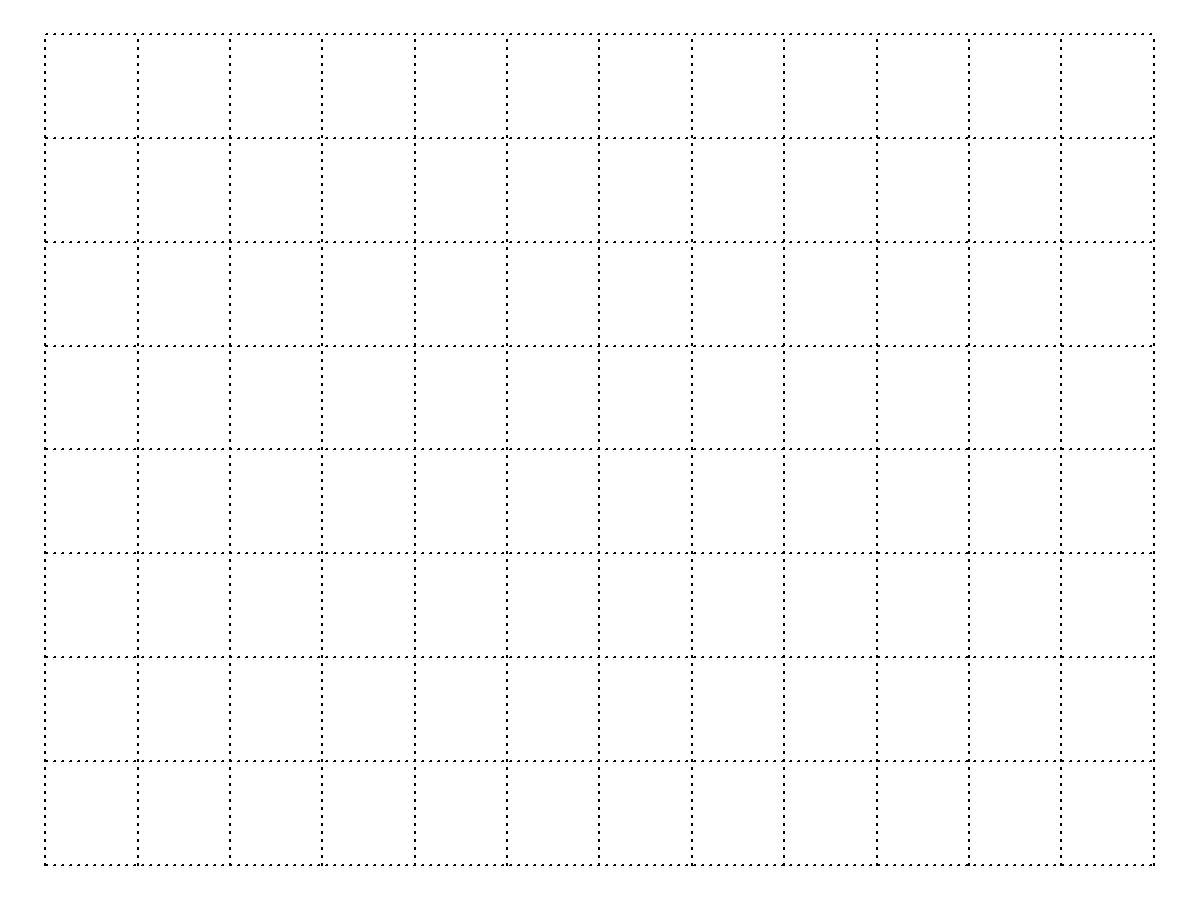
\includegraphics[width=0.5\linewidth]{graphics/empty_graph_wide_12}


 On the same axes, sketch the graph of $\arcsin(x)$, or $\sin^{-1}(x)$.

 \newpage
 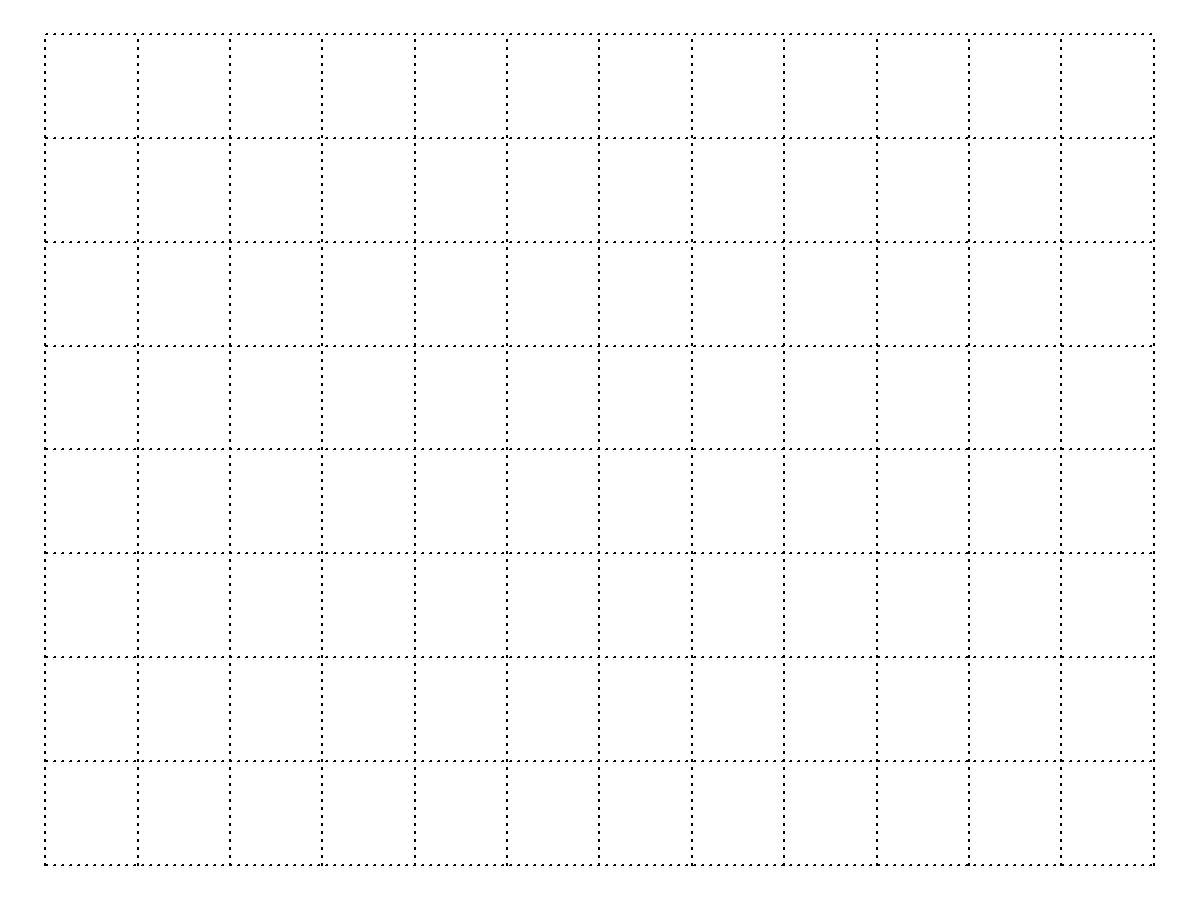
\includegraphics[width=0.5\linewidth]{graphics/empty_graph_wide_12}

 \problem What is the domain of $\arcsin(x)$?  \vspace{1in}

   What is the range of $\arcsin(x)$?
 \vspace{1in}

\newpage

\problem Sketch the graphs of $\arccos(x)$ and $\arctan(x)$. \\[2ex]

\begin{minipage}[t]{0.45\linewidth}
\begin{center}
Graph of $\arccos(x)$ \\
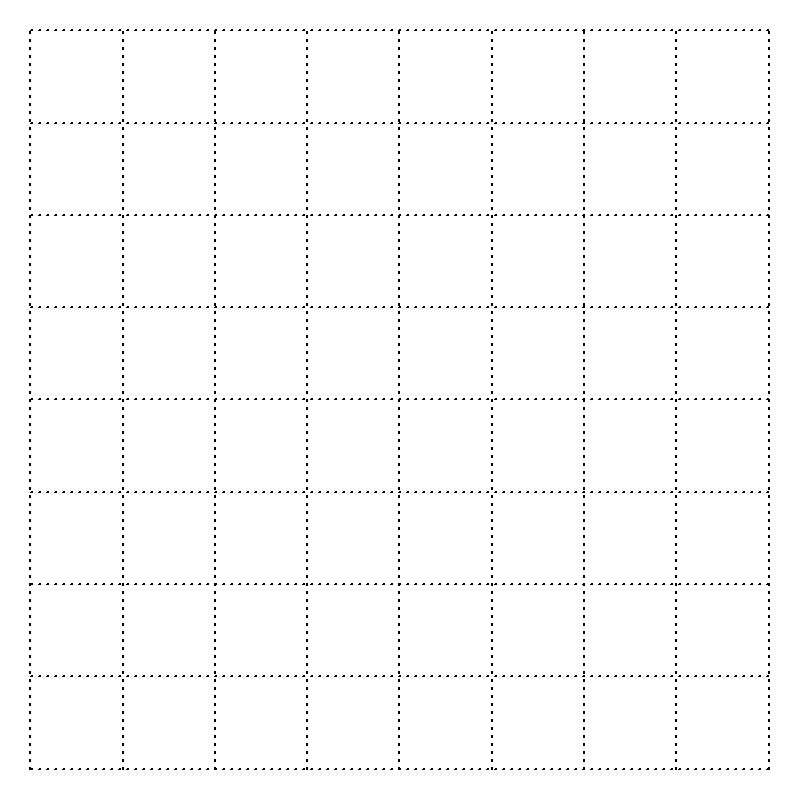
\includegraphics[width=0.9\linewidth]{graphics/empty_graph_square_8}
\end{center}
\end{minipage}
\hfill
\begin{minipage}[t]{0.45\linewidth}
\begin{center}
Graph of $\arctan(x)$ \\
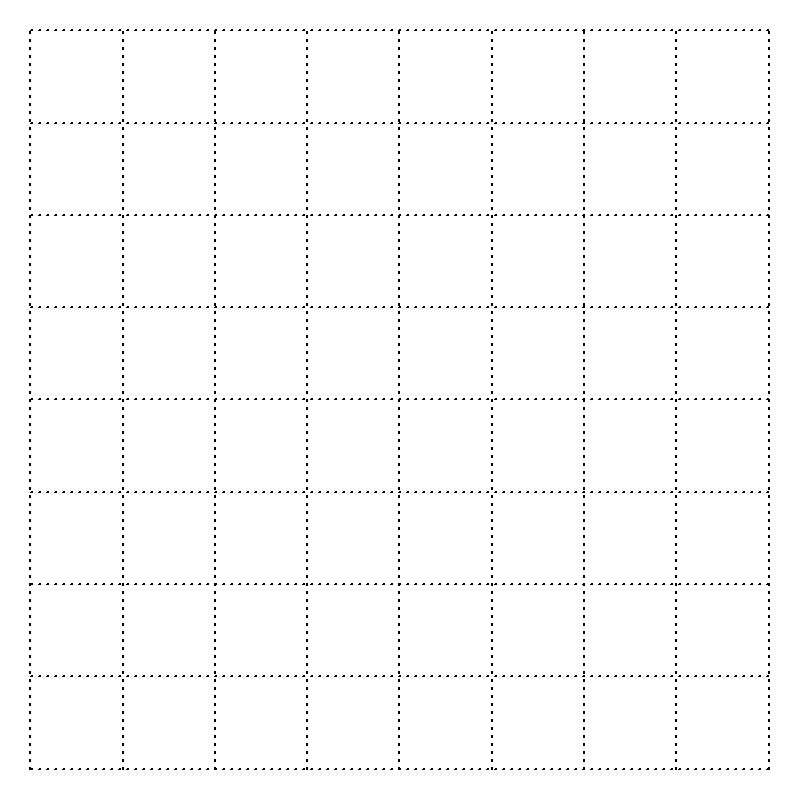
\includegraphics[width=0.9\linewidth]{graphics/empty_graph_square_8}
\end{center}
\end{minipage}
 \newpage

 \topic{Derivative of Inverse Trig Functions}

 \subsection*{Derivative of Inverse Trig Functions}
 \vsc \problem Simplify the expression $\sin (\arcsin x)$.

 \vspace{4cm} Differentiate both sides of this equation, using the
 chain rule on the left.  You should end up with an equation involving
 $\ds{ \diff \arcsin x}$.

 \vfill

 \newpage

 \problem  Solve for $\ds{\diff \arcsin x}$, and simplify the resulting
 expression by means of the formula
 $$
 \cos \theta = \sqrt{1-\sin^2 \theta}, 
 $$
 which is valid if $ \ds{\theta \in [-\frac{\pi}{2},\,\frac{\pi}{2}]}$.

 \vfill

\newpage
\begin{minipage}[t]{0.45\linewidth}
  \vspace{0pt} From this, we see that

 \begin{center}
  $\ds \diff \arcsin x =$ \hspace{2in}~
 \end{center}
\end{minipage}
\hfill
\begin{minipage}[t]{0.45\linewidth}
\vspace{0pt}
\begin{center}
Graph of $\arcsin(x)$ \\
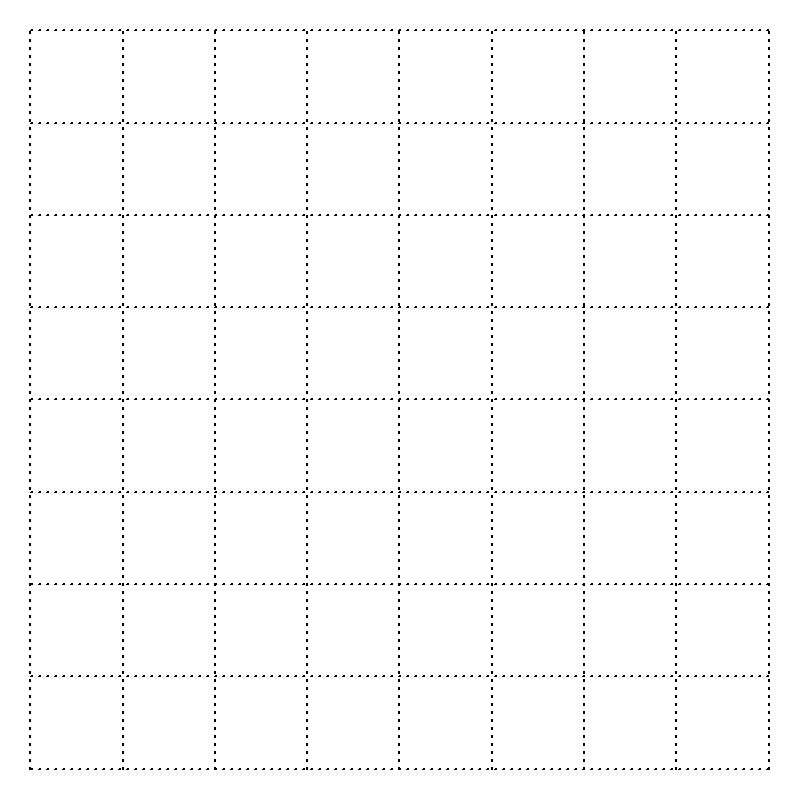
\includegraphics[width=0.7\linewidth]{graphics/empty_graph_square_8}

Graph of $\ds \ddx \arcsin(x)$ \\
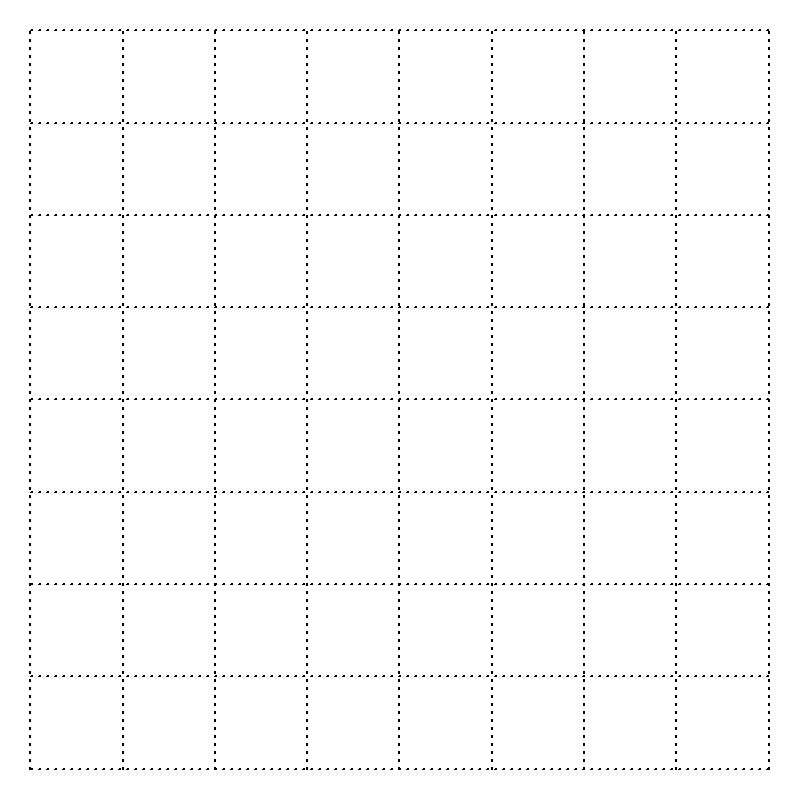
\includegraphics[width=0.7\linewidth]{graphics/empty_graph_square_8}
\end{center}
\end{minipage}

\newpage

Through a similar process, we can find the derivatives of all the
commonly used inverse trig functions.
\begin{boxnote}
$$ \ds \diff \arcsin( x) = \frac{1}{\sqrt{1-x^2}}$$ \\
$$ \ds \diff \arccos( x) = \frac{-1}{\sqrt{1-x^2}}$$ \\
$$ \ds \diff \arctan(x) = \frac{1}{1+x^2}$$
\end{boxnote}
\problem Note any common themes or differences, related to the earlier
trigonometric derivatives.

\newpage

\problem Evaluate the following derivatives.

$\ds \ddt{} \arcsin\left(\frac{x}{4}\right)$

\vfill

$\ds \ddx{} \arctan\left(e^{3x} \right)$

\vfill

  \end{document}

